\documentclass[aspectratio=169]{beamer}
\usetheme{metropolis}
\usepackage{appendixnumberbeamer}
\usepackage{booktabs, hyperref, textcomp}

\input{mgmt675-slides/mgmt675-style}

\title{Teaching with AI}
\author{Kerry Back}
\date{}

% Footer setup
\setbeamertemplate{frame numbering}[fraction]
\setbeamertemplate{footline}{
  \begin{beamercolorbox}[wd=\textwidth,ht=3ex,dp=1.5ex,leftskip=0.3cm,rightskip=0.3cm]{structure}
    UTEP, Feb 2026
    \hfill
    \insertframenumber{} / \inserttotalframenumber
  \end{beamercolorbox}
}

\begin{document}

\maketitle

% Overview slide
\begin{frame}{Questions}
  \begin{barenumerate}
  \item Should we have courses on AI, and, if so, what should they cover?
  \item To what extent and how should we incorporate AI into other courses?
  \item How can we use AI to enhance learning?
  \item How can we assess students?
  \end{barenumerate}

\end{frame}

\begin{frame}{One View}
  \begin{baritemize}
\item We should expect and encourage students to adopt AI as their go-to tool.

\item Rather than opening a spreadsheet, they should open a chat (or maybe a chat in a spreadsheet).

\item Every course should be about collaborating with AI to generate analysis, recommendations, and reports.  But AI should not take center stage.  It should just be the standard tool for analysis and reporting.

\item We have to assess students on whether they can defend the work they submit -- whether they can convince an audience that the reasoning and analysis is reliable.   It is possible that AI could help us in the assessment process.
  \end{baritemize}\end{frame}

\begin{frame}{A Course on AI}
\begin{baritemize}
  \item At present, we need courses focusing on AI.

\item Once AI has been integrated into the curriculum, we may not need stand-alone courses.

\item I will describe the course I am teaching (preparing to teach) at Rice: \href{https://mgmt675.kerryback.com}{mgmt675.kerryback.com}.  Much of it should soon be standard stuff that everyone does.

\item I'll come back to enhancing learning and also to using AI to simplify and accelerate our research and course development.
\end{baritemize}\end{frame}

% ========================================================================
% IMPORTED DECK: Course Introduction
% ========================================================================

\begin{frame}[plain]
\vfill
\begin{center}
{\fontsize{26}{30}\selectfont\bfseries\color{titlegray} Course Introduction}
\end{center}
\vfill
\end{frame}

\begin{frame}{From Makers to Checkers}
\begin{shadedbox}\centerline{Derek Waldron, JP Morgan Chief Analytics Officer}\end{shadedbox}

What we're working towards is that every employee will have their own personalized AI assistant; every process is powered by AI agents, and every client experience has an AI concierge.

You'll still have people at the top who are managing and have relationships with clients, but many, many of the processes underneath are now being done by AI systems.

Workers would shift from being creators of reports or software updates, or 'makers' ... to 'checkers' or managers of AI agents doing that work.
\end{frame}

\begin{frame}{The New Skills Landscape}
\begin{shadedbox}\centerline{Brookings Institute, 2025}\end{shadedbox}

As AI models begin to handle underwriting, compliance, and asset allocation, the traditional architecture of financial work is undergoing a fundamental shift.

As job descriptions evolve, so does the definition of financial talent. Excel is no longer a differentiator. Python is fast becoming the new Excel.

But technical skills alone will not cut it. The most in demand profiles today are those that speak both AI and finance.
\end{frame}

\begin{frame}{Why AI is Useful for Finance}
\begin{baritemize}
  \item AI can write code for financial analysis and building things (vibe coding)
  \item AI can generate Excel workbooks
  \item AI can draft reports (Word docs) and presentation decks (PowerPoint)
  \item AI can look up and answer questions about company practices, past company reports, communications, etc.
  \item AI can search the web, pull data from databases, or call APIs
  \item AI can analyze documents, contracts, or financial statements
  \item AI can automate repetitive tasks and workflows
  \item AI can communicate directly with clients (with strong controls)
\end{baritemize}
\end{frame}




% ========================================================================
% IMPORTED DECK: Collaborating with AI
% ========================================================================

\begin{frame}[plain]
\vfill
\begin{center}
{\fontsize{26}{30}\selectfont\bfseries\color{titlegray} Collaborating with AI}
\end{center}
\vfill
\end{frame}

\begin{frame}{The Mindset Shift}
\begin{baritemize}
  \item AI is not a search engine---it's a \alert{collaborator}
  \item Do not try to craft the ``perfect prompt''
  \item Instead: have a \alert{conversation}
  \item Think of AI as a capable colleague, not a vending machine
  \item The goal is \textit{iterative refinement}, not one-shot perfection
\end{baritemize}
\end{frame}


\begin{frame}{Ask the AI What It Can Do}
\begin{baritemize}
  \item AI systems know their own capabilities
  \item Ask: ``What information do you need from me to do this?''
  \item Ask: ``What are the different ways you could approach this?''
  \item Ask: ``What should I consider before we start?''
  \item Let the AI \alert{guide the conversation}---it often knows what questions to ask
\end{baritemize}

\vspace{0.5cm}
\begin{shadedbox}
\centerline{\textit{``I want to build a portfolio optimizer. What do you need to know to help me?''}}
\end{shadedbox}
\end{frame}


\begin{frame}{The Plan-Execute-Evaluate Cycle}
\begin{center}
\begin{tikzpicture}[scale=1.2]
  % Nodes
  \node[draw, rounded corners, fill=accentblue!20, minimum width=2.5cm, minimum height=1cm] (plan) at (0,2) {\textbf{Plan}};
  \node[draw, rounded corners, fill=accentblue!20, minimum width=2.5cm, minimum height=1cm] (execute) at (4,2) {\textbf{Execute}};
  \node[draw, rounded corners, fill=accentblue!20, minimum width=2.5cm, minimum height=1cm] (evaluate) at (2,0) {\textbf{Evaluate}};

  % Arrows
  \draw[->, thick, accentblue] (plan) -- (execute);
  \draw[->, thick, accentblue] (execute) -- (evaluate);
  \draw[->, thick, accentblue] (evaluate) -- (plan);
\end{tikzpicture}
\end{center}

\begin{baritemize}
  \item \textbf{Plan:} Define the task, gather requirements, outline approach
  \item \textbf{Execute:} Let AI do the work with your guidance
  \item \textbf{Evaluate:} Check results, identify gaps, refine
  \item Repeat until satisfied
\end{baritemize}
\end{frame}

\begin{frame}{Cross-Evaluation with Other AI Conversations}
\begin{baritemize}
  \item Start a \alert{new conversation} to evaluate the plan and output
  \item Even with the \textit{same model}, a fresh context can catch errors
  \item Ask the new conversation to review, critique, or verify
  \item Different phrasing may reveal blind spots
  \item Consider using a \textit{different model} for additional perspective
\end{baritemize}

\vspace{0.3cm}
\begin{shadedbox}
\textit{``I received this analysis from another session. Can you review it for errors or questionable assumptions?''}
\end{shadedbox}
\end{frame}


% ========================================================================
% IMPORTED DECK: AI with Code Execution
% ========================================================================

\begin{frame}[plain]
\vfill
\begin{center}
{\fontsize{26}{30}\selectfont\bfseries\color{titlegray} AI with Code Execution}
\end{center}
\vfill
\end{frame}

\begin{frame}{Benefit of Bundling Code Execution with AI}
\begin{baritemize}
  \item LLMs can write code, but writing is not the same as running
  \item Attaching a code execution tool enables:
  \begin{itemize}
    \item Data analysis with real calculations
    \item Visualizations and charts
    \item File processing (Excel, CSV, PDF)
    \item \alert{Iterative debugging---run, fix, repeat}
  \end{itemize}
  \item Transforms chatbots into computational tools
\end{baritemize}
\end{frame}

\begin{frame}{Vibe Coding}
\begin{shadedbox}\centerline{\textit{Fortune, Jan 29, 2026}}\end{shadedbox}
\vspace{0.5cm}

\textbf{Boris Cherny}, head of Claude Code at Anthropic:

\vspace{0.3cm}
\textit{``For me personally, it has been 100\% for two+ months now, I don't even make small edits by hand.''}

\vspace{0.3cm}
Across Anthropic, Cherny says \textit{``pretty much 100\%''} of code is AI-generated \ldots\ An Anthropic spokesperson said company-wide the figure is between 70\% and 90\%.

\end{frame}

\begin{frame}{Code Execution Locales}
\begin{columns}[T]
  \begin{column}{0.45\textwidth}
\begin{shadedbox}[title=\textbf{In the Cloud}]
\begin{itemize}\small
  \item ChatGPT, Claude, Gemini
  \item Upload files, ask questions
  \item Server-side sandbox
  \item No internet access (LLM can reach internet, but Python cannot)
\end{itemize}
\end{shadedbox}
\end{column}
\begin{column}{0.45\textwidth}
\begin{shadedbox}[title=\textbf{Locally}]
\begin{itemize}\small
  \item Cursor, GitHub Copilot, Claude Code
  \item LLM is in the cloud but code runs on your machine
  \item Full environment access
  \item Internet, databases, APIs
\end{itemize}
\end{shadedbox}
\end{column}

\end{columns}
\end{frame}


\begin{frame}{Claude.ai and Desktop: Two Code Execution Features}
\begin{columns}[T]
  \begin{column}{0.45\textwidth}
\begin{shadedbox}[title=\textbf{Artifacts}]
\begin{itemize}
  \item JavaScript in your browser
  \item Fast, lightweight
  \item Can save and publish artifacts
\end{itemize}
\end{shadedbox}
\end{column}
\begin{column}{0.45\textwidth}
\begin{shadedbox}[title=\textbf{Python Execution}]
\begin{itemize}
  \item Python/Bash on server
  \item Full linux environment
  \item \alert{Can install packages (pip)}
  \item No internet access
\end{itemize}
\end{shadedbox}
\end{column}
\end{columns}
\end{frame}

\begin{frame}{Claude Exercise}


\textit{``I'm uploading an Excel file with monthly returns for WMT, the excess market return (MKT-RF) and the risk-free rate (RF).  Calculate excess returns for WMT and regress on MKT-RF to estimate the beta of WMT.  Plot the data and the regression line.''}

\vspace{0.3cm}
Claude will write Python code, run it, show results, and let you download the chart.

\vspace{0.3cm}
\begin{shadedbox}
\centerline{\href{https://mgmt675.kerryback.com/files/betas.tex}{Data for Exercise}}
\end{shadedbox}
\end{frame}



\begin{frame}{Claude Artifacts}

\begin{baritemize}
  \item Interactive content in a panel next to the chat
  \item Codes in React/JavaScript---runs in your browser
  \item View, edit, and iterate in real-time
  \item \textbf{Save} artifacts to your account for later use
  \item \textbf{Publish} to create a public URL others can use (with charges to \alert{their account, not yours}.)
  \item Create and check once.  Use forever!
\end{baritemize}
\end{frame}

 \begin{frame}{Claude Artifact Exercise}

\textit{``Create an artifact that allows me to upload a csv file containing the return of a stock, the market excess return, and the risk-free rate over a given time period.  Compute excess returns of the stock and regress them on the market excess return.  Display the beta of the stock and a plot of the data with the regression line.''}

\vspace{0.3cm}
Claude creates an interactive artifact with file upload, regression calculations, and a chart---all running in your browser.
\end{frame}


% ========================================================================
% IMPORTED DECK: Spreadsheets and AI
% ========================================================================

\begin{frame}[plain]
\vfill
\begin{center}
{\fontsize{26}{30}\selectfont\bfseries\color{titlegray} Spreadsheets and AI}
\end{center}
\vfill
\end{frame}

\begin{frame}{AI Can Create Spreadsheets with Python}
\begin{baritemize}
  \item Python libraries like \texttt{openpyxl} create/modify Excel files
  \item AI writes Python code that:
  \begin{itemize}
    \item Inserts data values into cells
    \item Writes Excel formulas (e.g., \texttt{=SUM(A1:A10)})
    \item Applies formatting (fonts, colors, borders)
    \item Creates charts and pivot tables
  \end{itemize}
  \item Result: fully functional spreadsheet with \alert{live formulas}
\end{baritemize}
\end{frame}



\begin{frame}{Two Ways AI Interacts with Spreadsheets}
\begin{columns}[T]
  \begin{column}{0.45\textwidth}
\begin{shadedbox}[title=\textbf{Inside Excel (Add-ins)}]
\begin{itemize}\small
  \item Sidebar panel in Excel
  \item Sees your current workbook
  \item Modifies cells directly
  \item Context-aware suggestions
  \item Examples: Claude for Excel, Microsoft Copilot
\end{itemize}
\end{shadedbox}
\end{column}
\begin{column}{0.45\textwidth}
\begin{shadedbox}[title=\textbf{Outside Excel (Python)}]
\begin{itemize}\small
  \item Runs in terminal or IDE
  \item Creates/modifies .xlsx files
  \item You open result in Excel
  \item Full programming power
  \item Examples: Claude Code, ChatGPT
\end{itemize}
\end{shadedbox}
\end{column}
\end{columns}
\end{frame}

\begin{frame}{Claude for Excel Add-in}
\begin{baritemize}
  \item Runs Python in a server-side sandbox
  \item Reads multi-tab workbooks, explains calculations
  \item Modifies cells while preserving formula dependencies
  \item \alert{Does not require OneDrive}---works with local files
  \item Requires Claude Pro (\$20/month), Max, Team, or Enterprise plan
\end{baritemize}
\vspace{0.3cm}
\begin{shadedbox}
\centerline{
  \href{https://marketplace.microsoft.com/en-us/product/saas/wa200009404?tab=overview}{Claude Add-In for Excel}
}
\end{shadedbox}
\end{frame}




\begin{frame}{Exercise for Claude.ai or Claude Desktop}
  
\begin{shadedbox}
\centerline{``Create an Excel workbook to illustrate two-stage DCF analysis.''}
\end{shadedbox}
\end{frame}

\begin{frame}{Claude Skills}
\begin{baritemize}
  \item Claude ``skills'' are instructions that Claude reads when needed
  \item The \texttt{xlsx} skill instructs Claude to:
  \begin{itemize}
    \item Use Excel formulas instead of hardcoded values
    \item Apply professional formatting (color coding, number formats)
    \item Verify zero formula errors (\#REF!, \#DIV/0!, etc.)
    \item Follow financial modeling standards
  \end{itemize}
  \item Many available, easily customizable or created (just text files)
  \item \href{https://github.com/anthropics/claude-code/blob/main/skills/xlsx/skill.md}{View the full xlsx skill documentation}
\end{baritemize}
\end{frame}


% ========================================================================
% IMPORTED DECK: Creating Web Apps
% ========================================================================

\begin{frame}[plain]
\vfill
\begin{center}
{\fontsize{36}{40}\selectfont\bfseries\color{titlegray} Creating Web Apps}
\end{center}
\vfill
\end{frame}

\begin{frame}{Using Streamlit for Apps}
\begin{columns}[T]
\begin{column}{0.5\textwidth}
\begin{shadedbox}[title=\textbf{Streamlit Overview}]
\begin{itemize}\small
  \item Python library for web apps
  \item No HTML, CSS, or JavaScript needed
  \item Designed for data apps and dashboards
  \item Interactive widgets built-in
  \item Hot reload during development
\end{itemize}
\end{shadedbox}
\end{column}
\begin{column}{0.5\textwidth}
\begin{shadedbox}[title=\textbf{Perfect For}]
\begin{itemize}\small
  \item Data visualization dashboards
  \item Machine learning demos
  \item Financial analysis tools
  \item Interactive reports
  \item Chatbot interfaces
\end{itemize}
\end{shadedbox}
\end{column}
\end{columns}
\end{frame}

\begin{frame}{From Idea to Public App}
\begin{shadedbox}
The complete workflow to create and deploy a Streamlit app---all handled by Claude Code with simple natural language requests.
\end{shadedbox}
\vspace{0.3cm}
\begin{barenumerate}
  \item Create the Streamlit app
  \item Initialize a Git repository
  \item Create a GitHub repository
  \item Commit and push the code
  \item Deploy to Koyeb with auto-deploy
  \item Get your public URL
\end{barenumerate}
\vspace{0.3cm}
\begin{center}
\alert{Ask Claude to do each step---no commands to memorize}
\end{center}
\end{frame}


% ========================================================================
% IMPORTED DECK: Creating Custom Chatbots
% ========================================================================


\begin{frame}{Chatbots and Agents}
\vspace{0.5cm}
\begin{center}
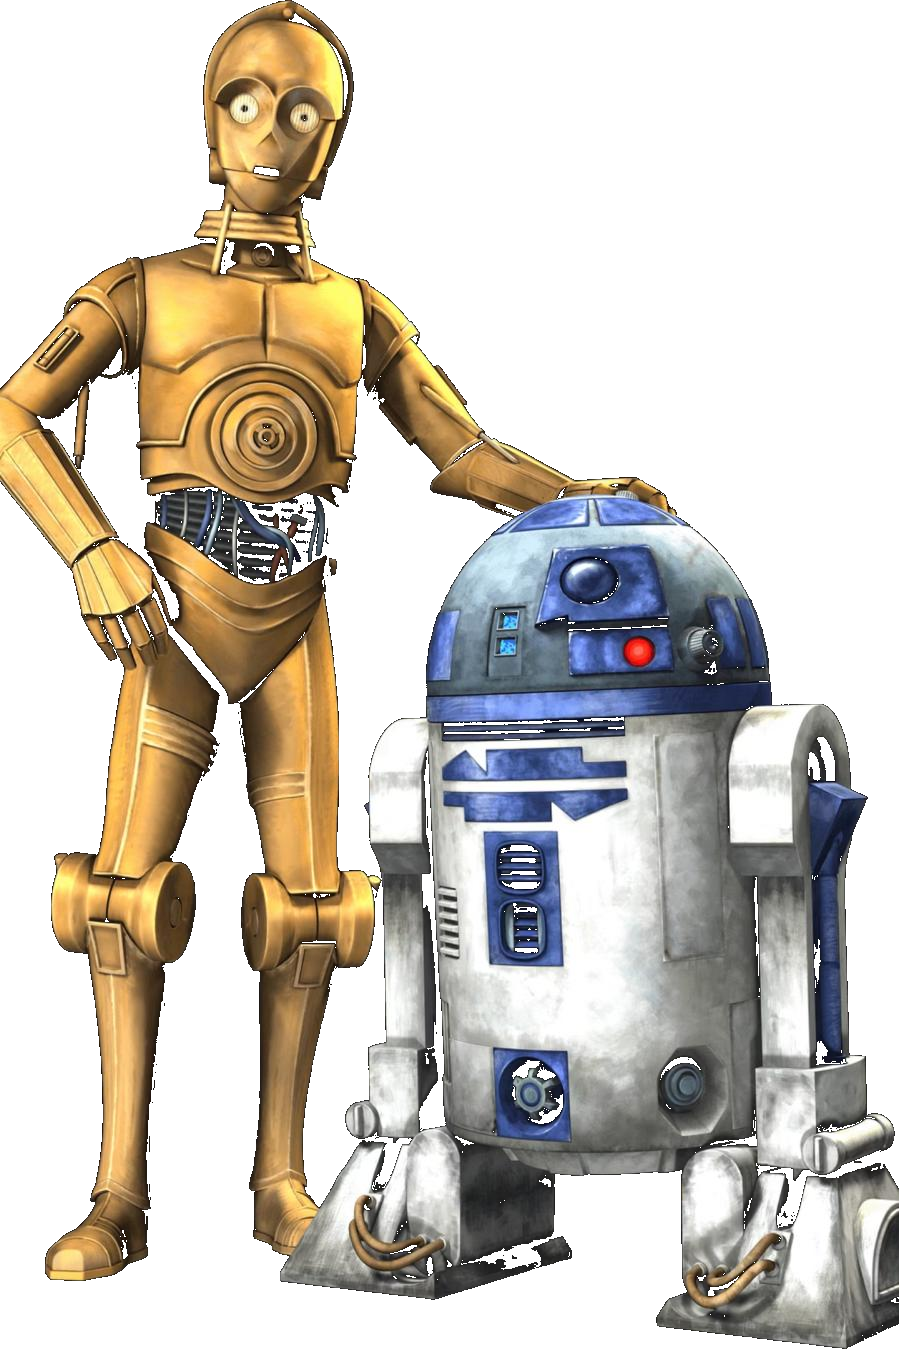
\includegraphics[height=0.7\textheight]{mgmt675-slides/images/c3po_r2d2_transparent.png}
\end{center}
\end{frame}



\begin{frame}{What is a Chatbot?}
\begin{columns}[T]
\begin{column}{0.5\textwidth}
\begin{shadedbox}[title=\textbf{Simple Definition}]
A chatbot is a program that:
\begin{enumerate}\small
  \item Accepts user input (prompt)
  \item Adds system prompt and sends to an LLM via API
  \item Displays the response
  \item Captures prompts and responses in a loop and sends history to LLM each time
\end{enumerate}
\end{shadedbox}
\end{column}
\begin{column}{0.5\textwidth}
\begin{baritemize}\small
  \item ChatGPT, Claude, Gemini are chatbots
  \item The LLM is the ``brain''
  \item The chatbot is the interface
  \item You can build your own!
\end{baritemize}
\end{column}
\end{columns}
\end{frame}


\begin{frame}{OpenRouter: One API, Many Models}
\begin{columns}[T]
\begin{column}{0.5\textwidth}
\begin{shadedbox}[title=\textbf{What is OpenRouter?}]
\begin{itemize}\small
  \item Unified API for 100+ models
  \item OpenAI, Anthropic, Google, Meta, etc.
  \item Single API key for all models
  \item Some models are free!
\end{itemize}
\end{shadedbox}
\vspace{0.3cm}
\begin{center}
\texttt{openrouter.ai}
\end{center}
\end{column}
\begin{column}{0.5\textwidth}
\begin{shadedbox}[title=\textbf{Free Models on Hugging Face}]
\begin{itemize}\small
  \item Hugging Face hosts open models
  \item OpenRouter provides free access
  \item Examples:
  \begin{itemize}\footnotesize
    \item \texttt{mistralai/mistral-7b-instruct:free}
    \item \texttt{meta-llama/llama-3-8b-instruct:free}
    \item \texttt{google/gemma-7b-it:free}
  \end{itemize}
\end{itemize}
\end{shadedbox}
\end{column}
\end{columns}
\end{frame}

\begin{frame}[fragile]{A Single API Call}
\begin{shadedbox}[title=\textbf{Basic Structure}]
\begin{verbatim}
import requests

response = requests.post(
    "https://openrouter.ai/api/v1/chat/completions",
    headers={"Authorization": f"Bearer {API_KEY}"},
    json={
        "model": "mistralai/mistral-7b-instruct:free",
        "messages": [{"role": "user", "content": prompt}]
    }
)
answer = response.json()["choices"][0]["message"]["content"]
\end{verbatim}
\end{shadedbox}
\end{frame}


\begin{frame}[fragile]{Message Format}
\begin{shadedbox}[title=\textbf{Messages Are a List of Dictionaries}]
\begin{verbatim}
messages = [
    {"role": "user", "content": "My name is Alice"},
    {"role": "assistant", "content": "Nice to meet you!"},
    {"role": "user", "content": "What's my name?"}
]
\end{verbatim}
\end{shadedbox}
\vspace{0.3cm}
\begin{columns}[T]
\begin{column}{0.5\textwidth}
\begin{shadedbox}[title=\textbf{Roles}]
\begin{itemize}\small
  \item \texttt{user}: Human messages
  \item \texttt{assistant}: LLM responses
  \item \texttt{system}: Instructions (special)
\end{itemize}
\end{shadedbox}
\end{column}
\begin{column}{0.5\textwidth}
\begin{baritemize}\small
  \item Each message has role + content
  \item Order matters (chronological)
  \item Send full list each API call
\end{baritemize}
\end{column}
\end{columns}
\end{frame}

\begin{frame}{The System Prompt}
\begin{shadedbox}
The \textbf{system prompt} is a special message that defines the chatbot's personality, knowledge, and behavior. It's the key to customization.
\end{shadedbox}
\vspace{0.3cm}
\begin{columns}[T]
\begin{column}{0.5\textwidth}
\begin{shadedbox}[title=\textbf{What It Does}]
\begin{itemize}\small
  \item Sets the chatbot's persona
  \item Defines its expertise
  \item Specifies response style
  \item Adds domain knowledge
  \item Sets guardrails/rules
\end{itemize}
\end{shadedbox}
\end{column}
\begin{column}{0.5\textwidth}
\begin{shadedbox}[title=\textbf{Placement}]
\begin{itemize}\small
  \item First message in the list
  \item Role is \texttt{system}
  \item Sent with every API call
  \item User never sees it directly
\end{itemize}
\end{shadedbox}
\end{column}
\end{columns}
\vspace{0.3cm}
\begin{shadedbox}
\centerline{\href{https://docs.anthropic.com/en/release-notes/system-prompts}{Anthropic's Published System Prompts for Claude}}
\end{shadedbox}
\end{frame}


\begin{frame}{What is an AI Agent?}
\begin{columns}
\begin{column}{0.4\textwidth}
\vskip\baselineskip
\begin{baritemize}\small
  \item A chatbot equipped with tools to perform actions beyond conversation.
  \item Code execution (Python, etc.)
  \item File generation (Excel, Word, PDF)
  \item Database access
  \item Web search and API calls
  \item System commands (copy, move files, etc.)
\end{baritemize}
\end{column}
\begin{column}{0.6\textwidth}
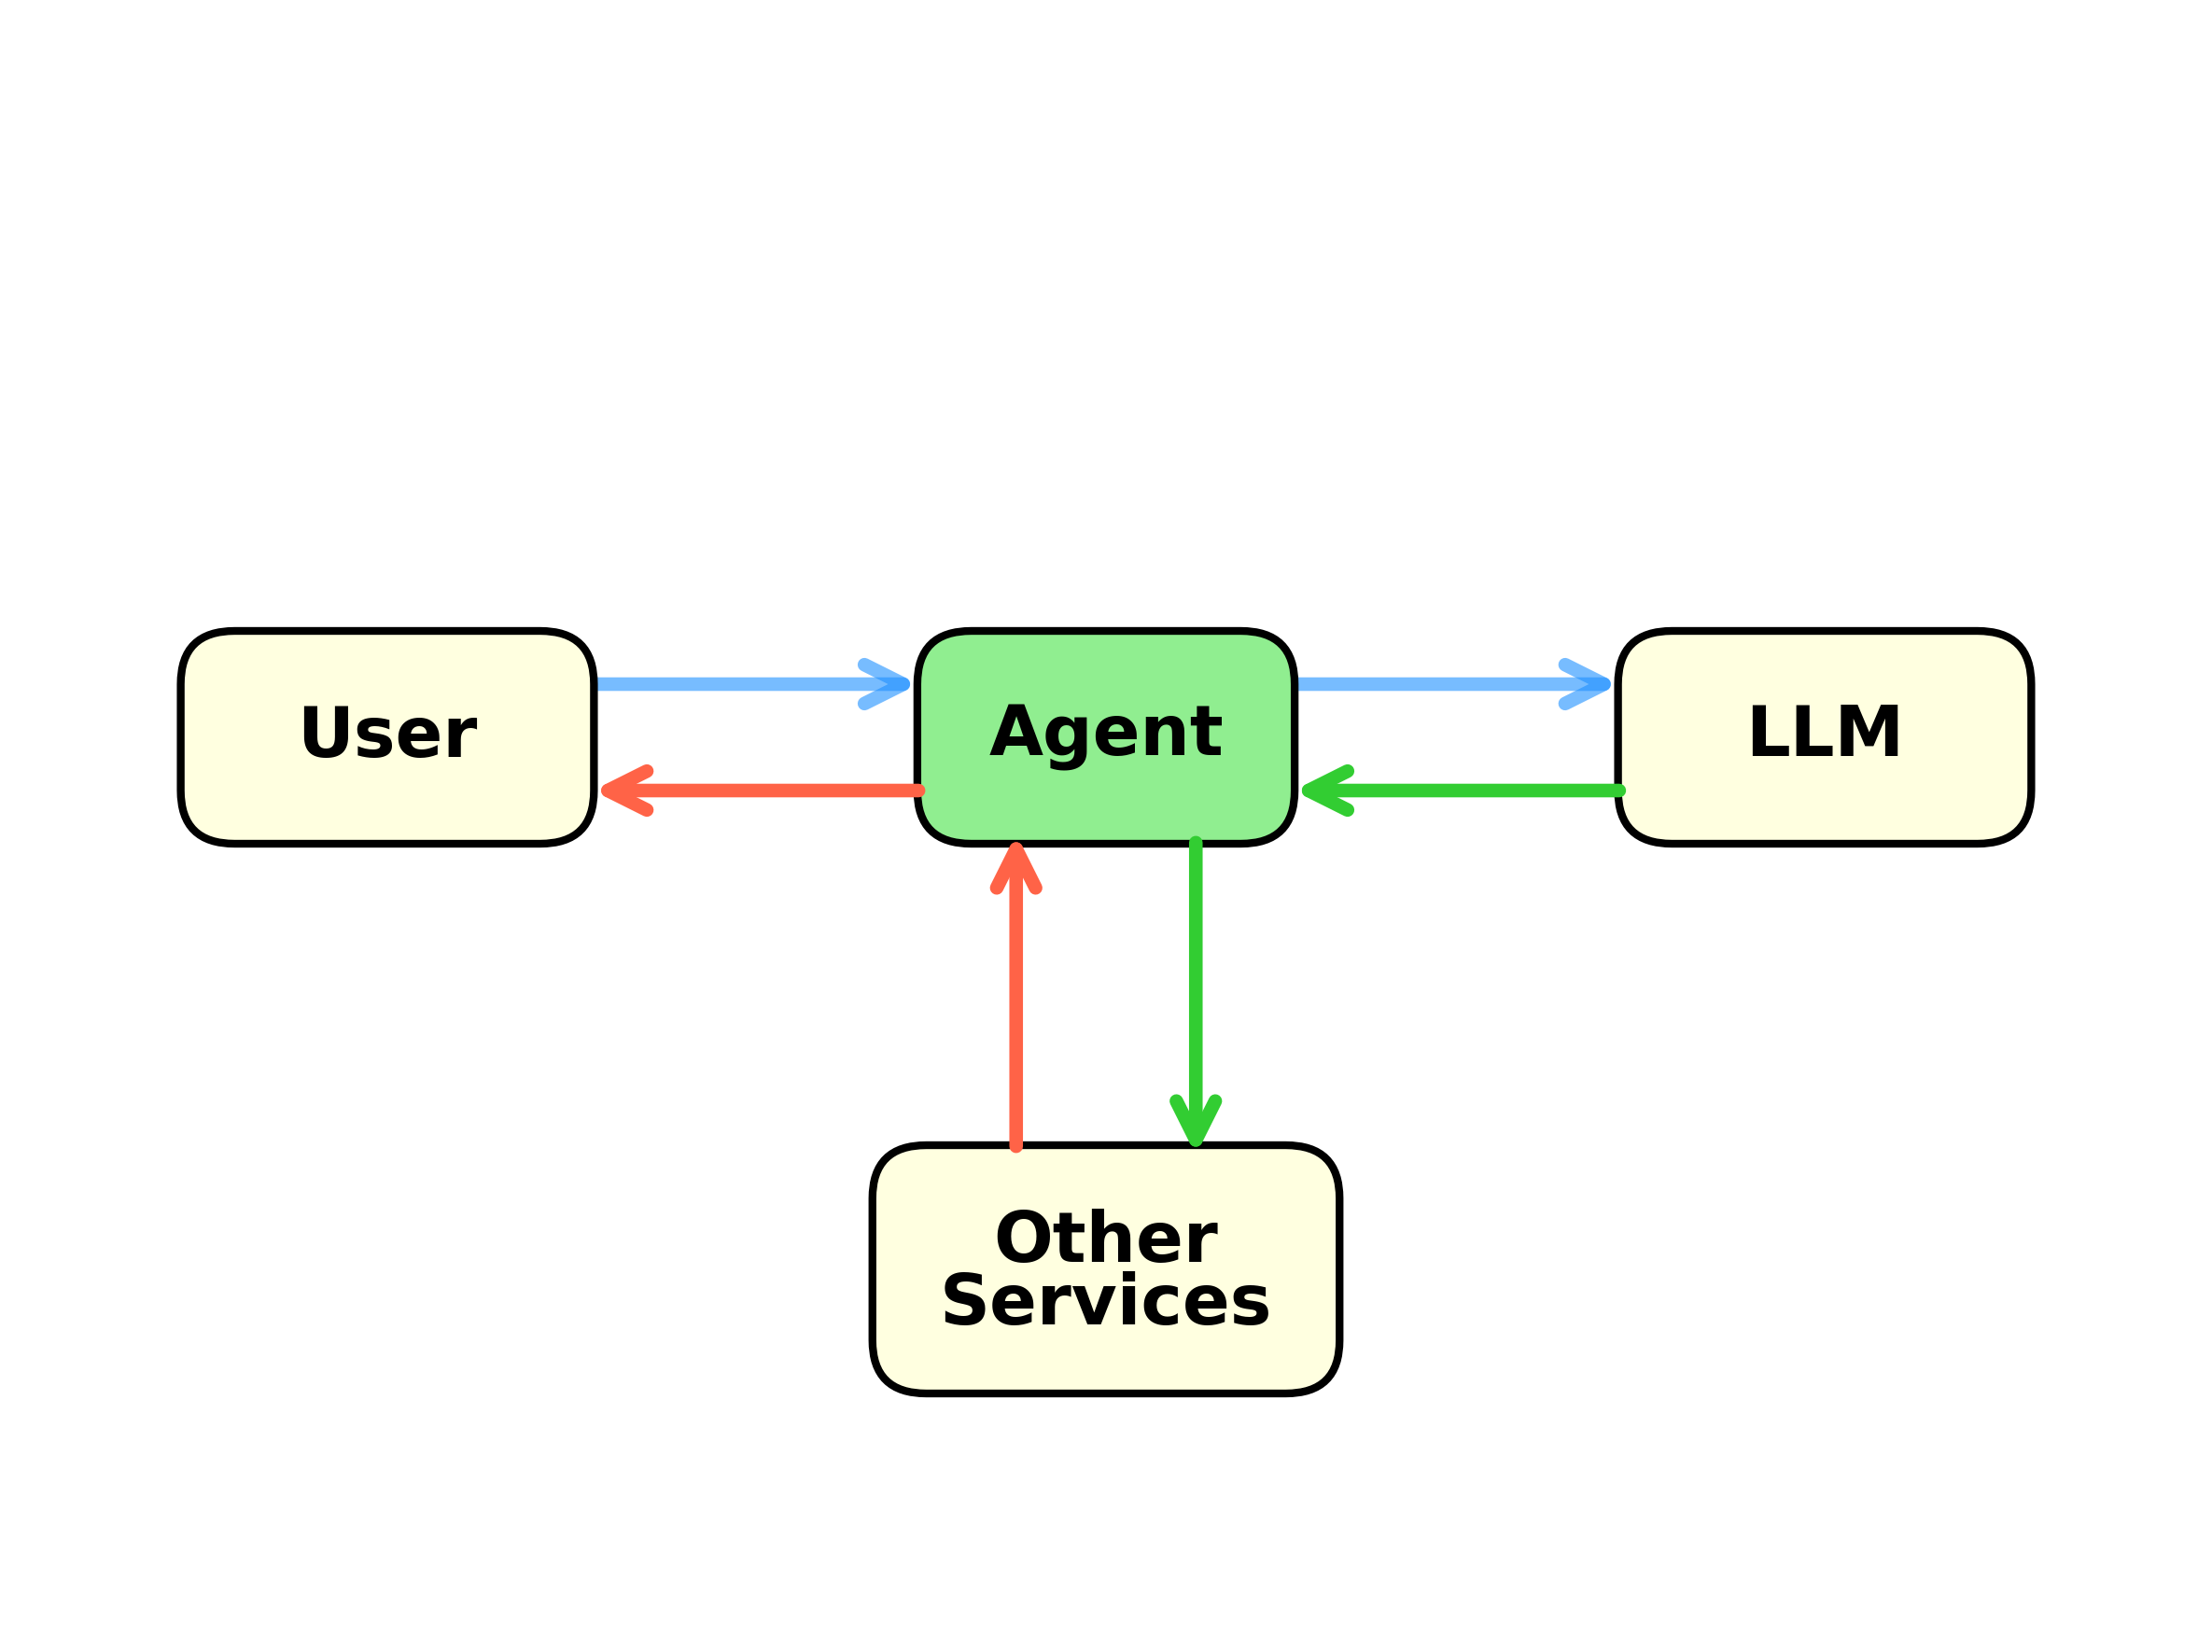
\includegraphics[width=\textwidth]{mgmt675-slides/images/slide6_img1.png}
\end{column}
\end{columns}
\end{frame}




\begin{frame}{What Are Tools?}
\begin{shadedbox}
\textbf{Tools} are functions the agent can call to interact with the outside world.
\end{shadedbox}
\vspace{0.3cm}
\begin{columns}[T]
\begin{column}{0.5\textwidth}
\begin{shadedbox}[title=\textbf{Example Tools}]
\begin{itemize}\small
  \item Execute SQL queries
  \item Run Python code
  \item Read/write files
  \item Search the web
  \item Send emails
  \item Call APIs
\end{itemize}
\end{shadedbox}
\end{column}
\begin{column}{0.5\textwidth}
\begin{shadedbox}[title=\textbf{How Tools Work}]
\begin{enumerate}\small
  \item LLM decides to use a tool
  \item Returns tool name + parameters
  \item Agent executes the tool
  \item Result sent back to LLM
  \item LLM continues reasoning
\end{enumerate}
\end{shadedbox}
\end{column}
\end{columns}
\end{frame}


\begin{frame}{How Coordination Works}
\begin{shadedbox}
The agent combines \textbf{LLM responses} with \textbf{pre-programmed logic} to decide the next action.
\end{shadedbox}
\vspace{0.3cm}
\begin{columns}[T]
\begin{column}{0.5\textwidth}
\begin{shadedbox}[title=\textbf{LLM Decides}]
\begin{itemize}\small
  \item Which tool to call next
  \item What parameters to pass
  \item When the task is complete
  \item What to ask the user
\end{itemize}
\end{shadedbox}
\end{column}
\begin{column}{0.5\textwidth}
\begin{shadedbox}[title=\textbf{Code Decides}]
\begin{itemize}\small
  \item If tool\_call $\rightarrow$ execute tool
  \item If error $\rightarrow$ retry or report
  \item If question $\rightarrow$ prompt user
  \item If done $\rightarrow$ return response
\end{itemize}
\end{shadedbox}
\end{column}
\end{columns}
\vspace{0.3cm}
\begin{center}
\alert{The agent is part LLM intelligence, part traditional programming}
\end{center}
\end{frame}



\begin{frame}{data-portal.rice-business.org}
\begin{columns}
\begin{column}{0.4\textwidth}
  \vskip\baselineskip
\begin{baritemize}\small

  \item Prompt + System Prompt $\rightarrow$ LLM
  \item LLM $\rightarrow$ SQL code or a question for the user
  \item Agent $\rightarrow$ SQL code to database or $\rightarrow$ question to the user
  \item Eventually, SQL code $\rightarrow$ database
  \item Database $\rightarrow$ data or error message
  \item Error message $\rightarrow$ LLM
  \item Eventually data $\rightarrow$ user
\end{baritemize}
\end{column}
\begin{column}{0.6\textwidth}
\vspace{1cm}
\begin{shadedbox}\begin{center}
  Visit \href{https://data-portal.rice-business.org}{data-portal.rice-business.org}
  \newline Get access token, Log in, Ask for data
\end{center}\end{shadedbox}
\vspace*{-2\baselineskip}
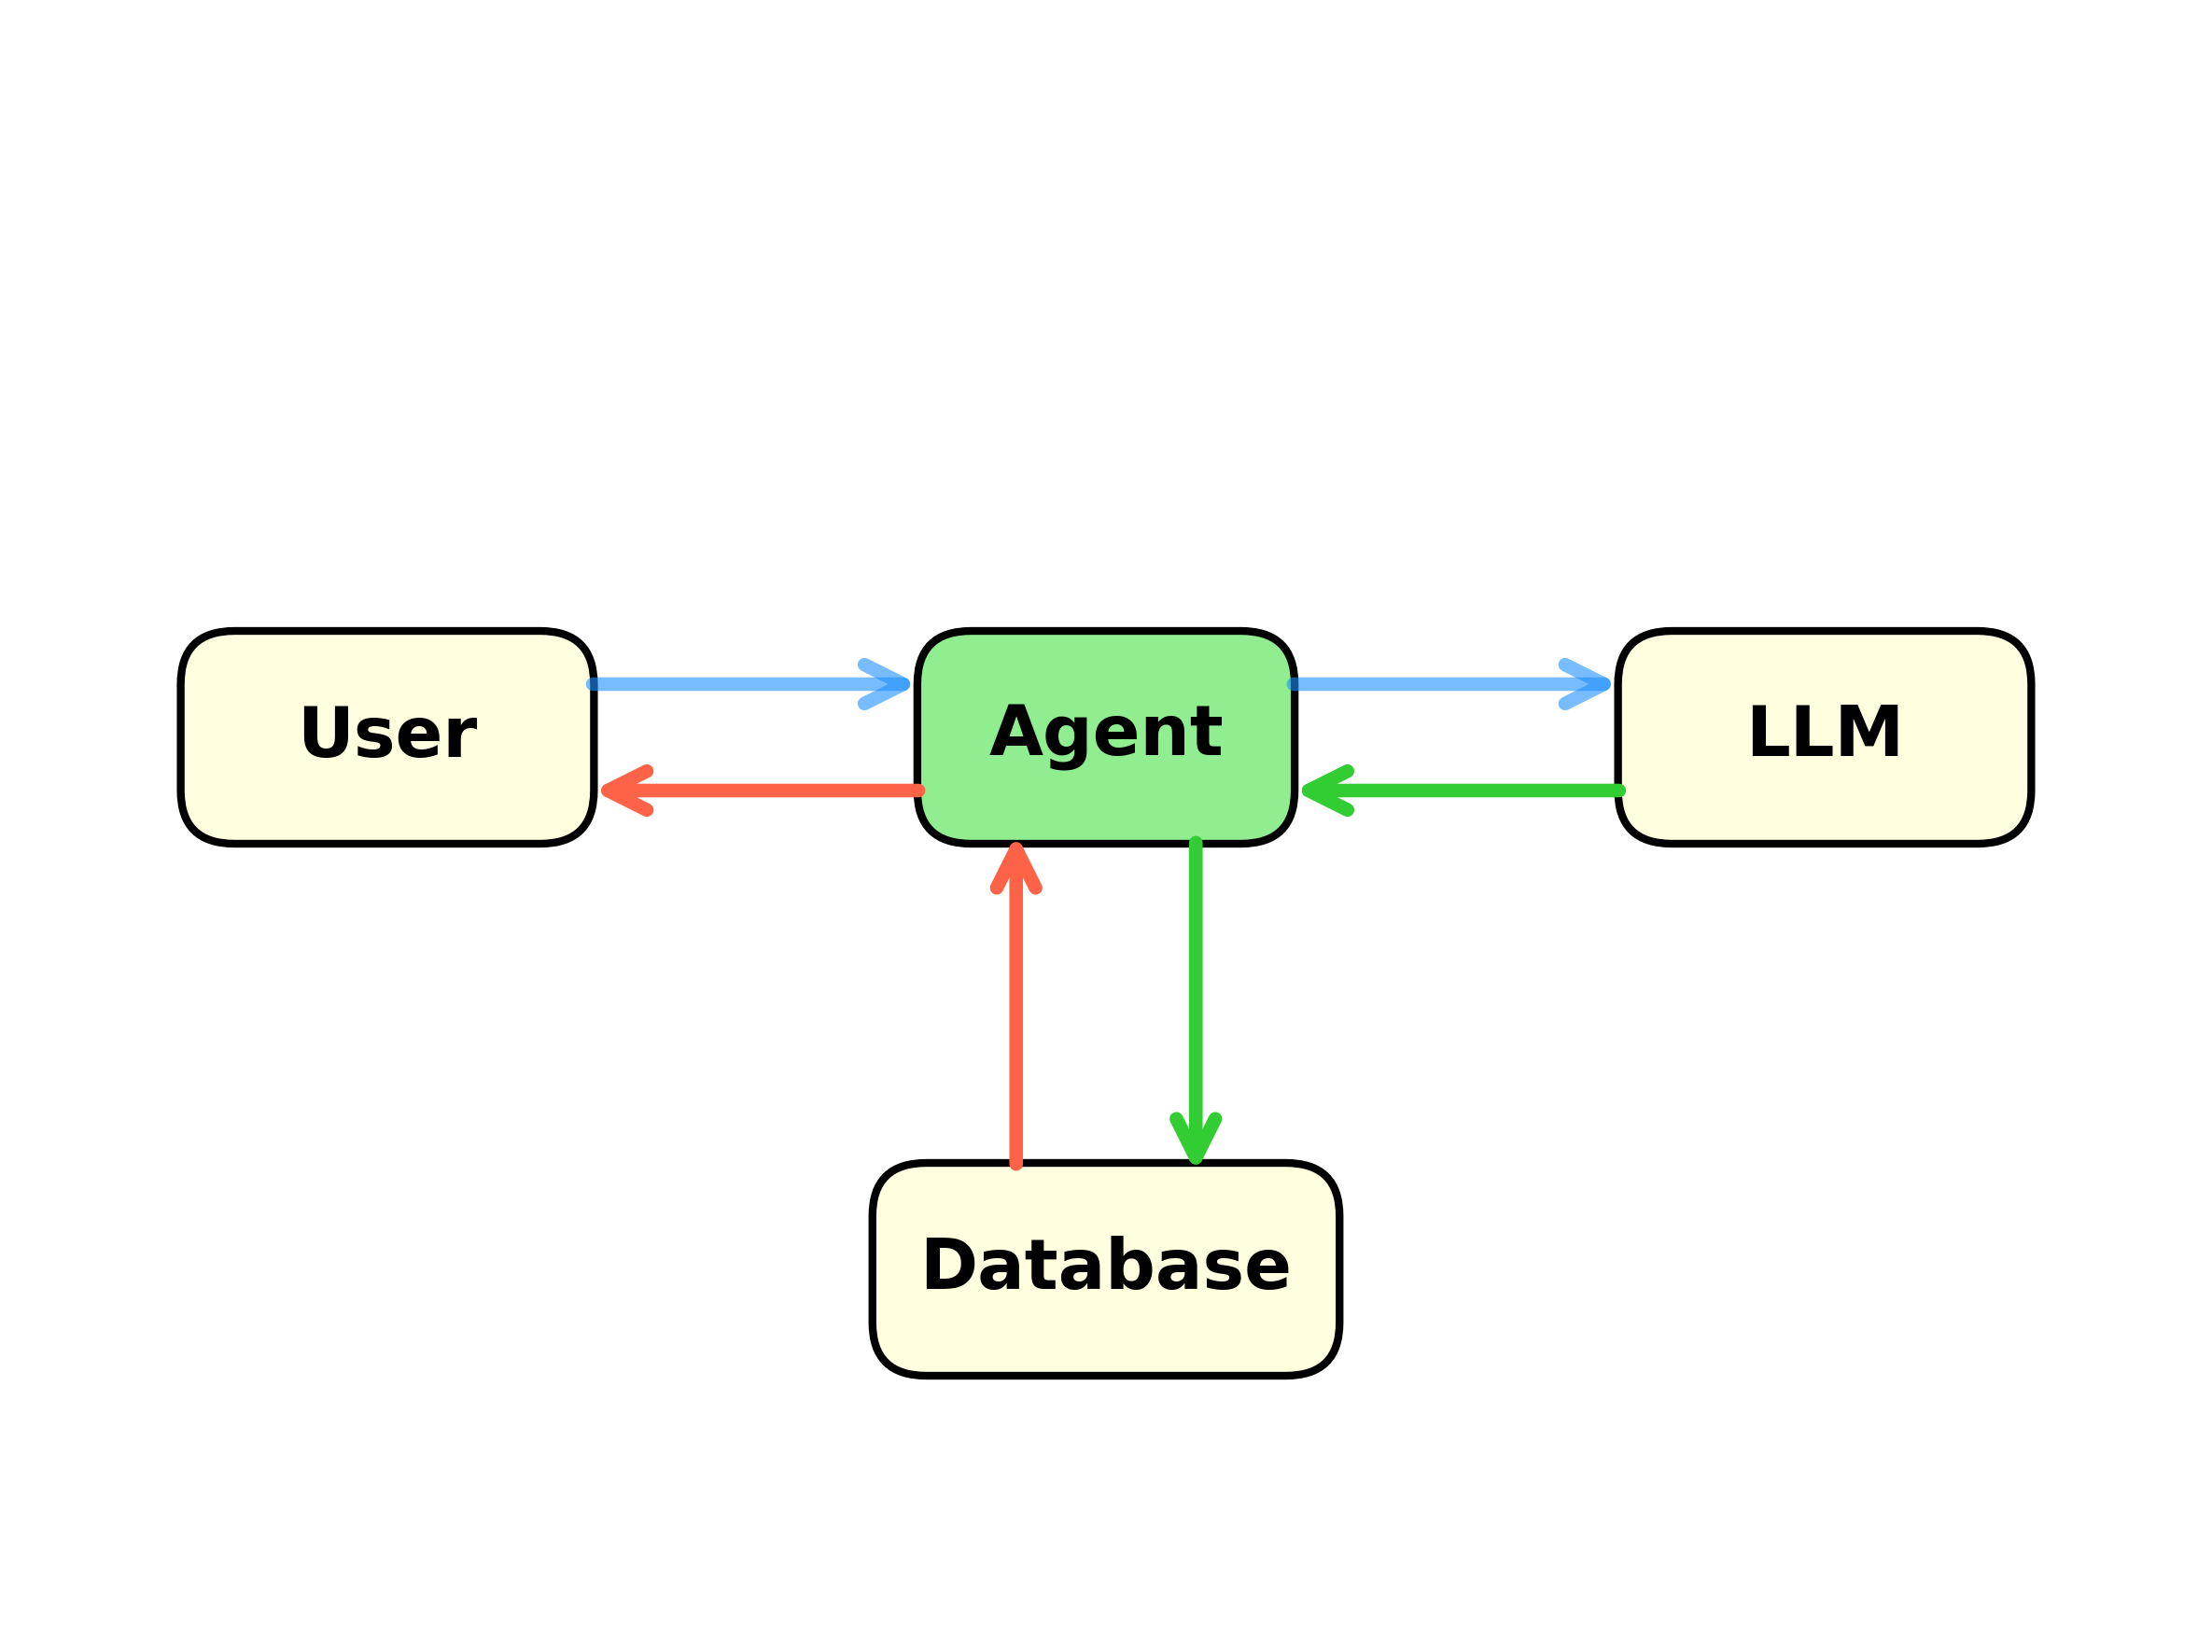
\includegraphics[width=\textwidth]{mgmt675-slides/images/agent_database.png}
\end{column}
\end{columns}
\end{frame}







%========================================================================
% IMPORTED DECK: Local Execution: Python, Claude Code, VS Code
% ========================================================================

\begin{frame}[plain]
\vfill
\begin{center}
{\fontsize{26}{30}\selectfont\bfseries\color{titlegray} Local Execution: Python,\\ Claude Code, VS Code}
\end{center}
\vfill
\end{frame}
\begin{frame}{Course Install Files}
\begin{baritemize}
  \item Python 3.12, VS Code, Git, Quarto, TinyTeX, Node.js, Claude Code
  \item VS Code extensions: Python, Jupyter, Claude Code, Quarto, LaTeX Workshop, GitHub Copilot
 \item Command line interfaces for GitHub, Koyeb
\end{baritemize}
\vspace{0.3cm}
\begin{shadedbox}
\centering\href{https://kerryback.com/mgmt675/software.html}{Class Software Installer}
\end{shadedbox}
\end{frame}

\begin{frame}{Opening a Folder in VS Code}
\begin{baritemize}
  \item VS Code works with \alert{folders}, not individual files
  \item File $\rightarrow$ Open Folder $\rightarrow$ select your project folder
  \item The folder appears in the Explorer sidebar (left panel)
  \item All files in the folder are accessible
  \item This is your workspace for a project
\end{baritemize}
\vspace{0.3cm}
\begin{shadedbox}
\centering Tip: Create a dedicated folder for course work
\end{shadedbox}
\end{frame}

\begin{frame}{Opening Claude Code}
\begin{baritemize}
  \item \textbf{Spark icon}: Click the spark icon in the top-right corner of any open file
  \item \textbf{Status bar}: Click ``Claude Code'' in the bottom-right corner
  \item \textbf{Command Palette}: Ctrl+Shift+P $\rightarrow$ type ``Claude Code''
  \item \textbf{Keyboard shortcut}: Cmd+Esc (Mac) / Ctrl+Esc (Windows)
\end{baritemize}
\end{frame}

\begin{frame}{What Claude Code Can Do}
\begin{baritemize}
  \item Explain code and answer questions
  \item Write new code from descriptions
  \item Fix errors and debug problems
  \item Edit files (with your approval)
  \item \alert{Run commands in the terminal}
  \item Create and modify Jupyter notebooks, Python scripts, LaTeX files, \ldots
\end{baritemize}
\end{frame}


\begin{frame}{Exercise: Estimating Betas}
\begin{baritemize}
\item In VS Code, open the folder containing betas.xlsx (or copy it into the folder currently open in VS Code)
\item  Ask Claude Code to compute WMT's excess returns and run a regression to estimate its beta.  
\item Ask for a Word doc containing a scatterplot of the data with the regression line and a discussion of why the beta is what it is.
\end{baritemize}

\begin{center}
\begin{shadedbox}[width=0.7\textwidth]
\centering\href{https://kerryback.com/mgmt675/files/betas.xlsx}{Data for Exercise}
\end{shadedbox}
\end{center}
\end{frame}

\begin{frame}{Exercise: Aggregating Tables}
\begin{baritemize}
\item Download aggregation.zip into the folder open in VS Code.
\item Extract all the workbooks in the zip file.
\item Each workbook contains a table with similar data.  Some tables are missing some columns and the names of some of the columns vary somewhat across the tables.  Ask Claude Code to combine the tables into a single table, to include all columns, and to reconcile the varying names.
\end{baritemize}

\begin{center}
\begin{shadedbox}[width=0.7\textwidth]
\centering\href{https://kerryback.com/mgmt675/files/aggregation.zip}{Data for Exercise}
\end{shadedbox}
\end{center}
\end{frame}



\begin{frame}{Exercise: Mean-Variance App}
\begin{shadedbox}
Build and deploy a Streamlit app for mean-variance portfolio optimization.
\end{shadedbox}
\vspace{0.3cm}
\begin{columns}[T]
\begin{column}{0.5\textwidth}
\begin{shadedbox}[title=\textbf{User Inputs}]
\begin{itemize}\small
  \item Risk-free rate
  \item Number of risky assets
  \item Expected returns (means)
  \item Standard deviations
  \item Correlation matrix
\end{itemize}
\end{shadedbox}
\end{column}
\begin{column}{0.5\textwidth}
\begin{shadedbox}[title=\textbf{App Outputs}]
\begin{itemize}\small
  \item Tangency portfolio weights
  \item Downloadable image of:
  \begin{itemize}\footnotesize
    \item Frontier of risky assets
    \item Capital allocation line
  \end{itemize}
\end{itemize}
\end{shadedbox}
\end{column}
\end{columns}
\end{frame}

\begin{frame}{AI for Class Preparation and Research}
Some Claude Code prompts:

\begin{baritemize}
\item Using this data \ldots compute these statistics \ldots and put them in a latex table like this \ldots and insert them in my paper in \ldots
\item Using this data \ldots generate figures like this \ldots and insert them in \ldots
\item I don't like the way I worded things in this paragraph \ldots Please clean it up.
\item I want to add a slide to my lecture about \ldots It should say \ldots in bullet points
\item Use the Google API to get an image that represents \ldots and insert it into  \ldots
\item Make this edit to \ldots and then render, commit, and push to update this website \ldots
\item Build my latex file.  Find and fix any errors.
\item Using sympy, simplify this integral \ldots
\end{baritemize}
\end{frame}

\begin{frame}{Enhancing Learning: NotebookLM}
\begin{baritemize}
\item In addition to using AI for financial analysis, students should use AI to learn.
\item Can ask them to chat with a chatbot about a subject in lieu of reading assignments.
\item Can use retrieval-augmented generation (chatbot answers questions from specific sources)
\item NotebookLM is an easy way to do this.  Example:  \href{https://notebooklm.google.com/notebook/701244f5-4833-4217-875d-96380578825b}{chatbot about Pricing and Hedging Derivative Securities (online textbook by Back, Liu, and Loewenstein)}
\item NotebookLM provides other tools, including AI-generated slide presentations.  Example: \href{https://mgmt638.kerryback.com/videos/Kapadia_Ostdiek_Weston_Zekhnini_JFQA_2019.mp4}{Presentation of Getting Paid to Hedge: Why Don't Investors Pay
a Premium to Hedge Downturns? by Kapadia, Ostdiek, Weston, and Zekhnini, JFQA, 2019}
\end{baritemize}
\end{frame}
\end{document}
